
\section{Procedure}
\label{procedure}
I due algoritmi \ScanTrans e \MergeTrans vengono scomposti in diversi componenti, ognuno dei quali viene valutato nelle performance e testato separatamente. 

\subsection{Scan}
\label{scan}
Questa operazione prende in input un vettore $A = (a_0, a_1, ..., a_n)$ e ritorna un vettore $B=(I, a_0, a_0 \oplus a_1, ..., a_0 \oplus a_1 \cdots \oplus a_{n-1})$ con $\oplus$ è un'operazione binaria il cui elemento identità è $I$. Nel nostro caso l'operazione è la somma. 

L'algoritmo apparentemente sembra difficile da parallelizzare in quanto il risultato di ogni elemento dipende da tutti i gli elementi precedenti. Diverse soluzioni sono state proposte tra cui l'\emph{algoritmo di Blelloch}. Il suo funzionamento in due fasi è illustrato in Figura~\ref{scan_blelloch} e dettagliatamente discusso in \cite{scan}.

\begin{figure}[H]
	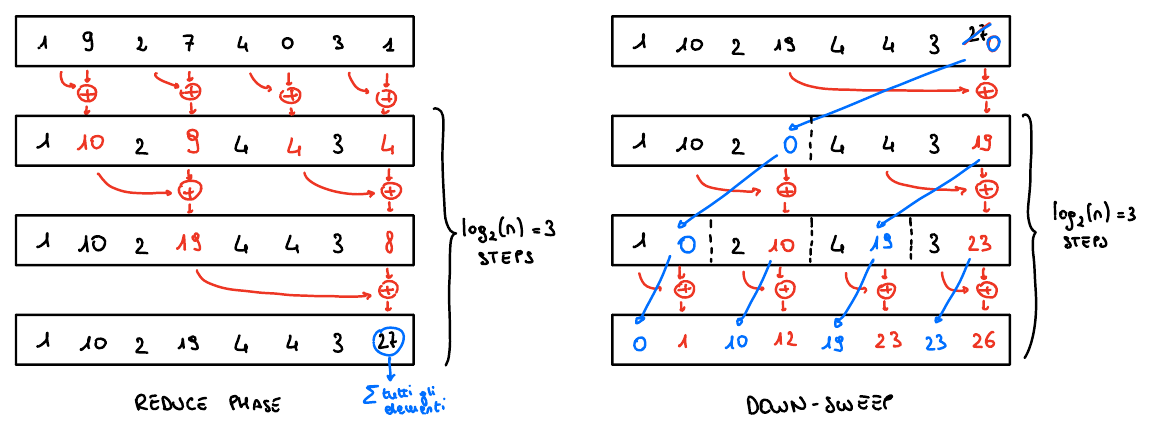
\includegraphics[scale=0.3]{scan.png}
	\caption{Algoritmo di Blelloch}
	\label{scan_blelloch}
\end{figure}

L'implementazione prevede che se l'intero vettore riesce ad essere memorizzato all'interno della shared memory di $N$ elementi, allora possiamo calcolare scan con una singola chiamata a kernel. 

Nel caso questo non sia possibile, l'operazione di scan viene segmentata, applicata separatamente a blocchi di $N$ elementi. Successivamente si mantiene un vettore di somme (vettore degli ultimi elementi del blocco), si applica ricorsivamente \emph{scan} su esso e si sommano gli offset ottenuti all'intero vettore di partenza. 

\subsection{Segmented sort}
\label{seg-sort}
Questa operazione prende in input un vettore di lunghezza $n$ ed un intero $\BlockSize$. Il vettore viene diviso in segmenti di lunghezza $\BlockSize$. Gli elementi di ogni segmento vengono permutati in modo che siano ordinati stabilmente. L'intero segmento deve rientrare nella shared memory.  

\begin{figure}[H]
\centering
	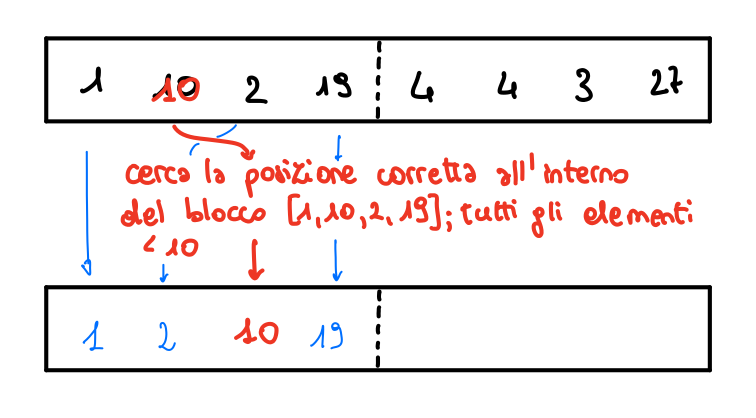
\includegraphics[scale=0.15]{segmented_sort.png}
	\caption{Segmented Sort}
	\label{segmented_sort}
\end{figure}

Una volta caricato il blocco in shared memory, la $i$-esima thread del blocco è incaricata di trovare la posizione corretta dell'$i$-esimo elemento all'interno del segmento, ed assegnarlo a tale posizione. L'algoritmo viene illustrato in Figura~\ref{segmented_sort}. 

L'ordinamento deve essere stabile quindi la posizione dell'$i$-esimo elemento di valore $y$ è dato dal numero di elementi $<y$, sommati al numero degli elementi $=y$ per indici $<i$. 

La dimensione ideale del blocco pari a $128$ elementi (caso interi a 32bit), ed è stata trovata empiricamente:
\begin{figure}[H]
    \centering
    \begin{tabular}{SS}
    \toprule
    \textbf{Thread per blocco} & \textbf{Performance (\si{\milli\second})} \\ \midrule
    64 & 9999.0 \\
    128 & 999.5 \\
    256 & 99.0 \\ \bottomrule
    \end{tabular}
    \caption{Performance su array di $2\cdot 10^7$ elementi}
\end{figure}

\subsection{Merge}
\label{merge}
L'operazione di \emph{merge} trasforma un vettore diviso in segmenti di dimensione $\BlockSize$ nel quale gli elementi ogni segmento sono ordinati, in un vettore diviso in segmenti ordinati di dimensione $2 \BlockSize$, ognuno dei quali è l'unione di una coppia di blocchi contigui. 

Differenziamo il caso in cui il blocco di dimensione $\BlockSize$ rientri o meno nella shared memory. 

\subsection{Merge small}

In questo caso una coppia di blocchi rientra completamente nella shared memory. In modo analogo a quanto fatto per l'operazione di \emph{segmented sort}, abbiamo un numero di thread per blocco pari a $\BlockSize$ nel quale l'$i$-esimo thread è incaricato di calcolare la posizione dell'$i$-esimo elemento. 

In questo caso la posizione dell'$i$-esimo elemento del blocco di sinistra è $i+j$ con $j$ posizione dell'elemento all'interno del blocco di destra, trovato attraverso una ricerca binaria in quanto i blocchi sono ordinati (differentemente da quanto avviene per il segmented sort). Analogamente lo stesso avviene per gli elementi del blocco di destra. 

A parità di valore, gli elementi del blocco di sinistra hanno indice minore di quelli di destra. 

\subsection{Merge big}

\begin{figure}[t]
    \centering
	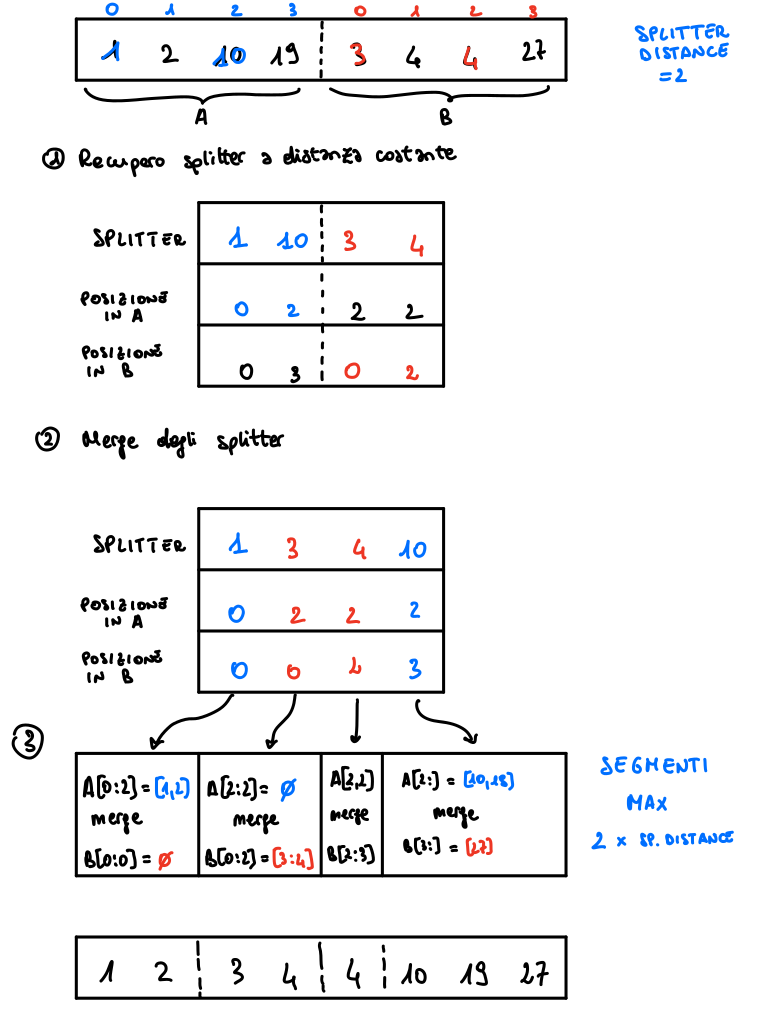
\includegraphics[scale=0.3]{merge_big.png}
	\caption{Merge big}
	\label{merge_big}
\end{figure}

Questo secondo algoritmo è illustrato in Figura~\ref{merge_big} ed originariamente preso da \cite{mergebig}. Applicando sempre \emph{merge small}, oltre che rinunciare alla shared memory, ogni thread del blocco dovrebbe lavorare su più di un elemento, aumentando la complessità della procedura. 

L'algoritmo proposto funziona nel seguente modo:
\begin{enumerate}
    \item recuperiamo dal vettore degli elementi segnaposto detti \emph{splitter} presi a distanza costante e pari ad $\SplitterDistance$; \\
    per ogni coppia di segmenti da mergiare ho una coppia di blocchi di splitter, trovo la posizione di ogni splitter all'interno del blocco di destra ($A$) e di sinistra ($B$);
    \item applico \emph{merge} ricorsivamente sugli array di splitter;
    \item gli indici associati agli splitter dividono la coppia di blocchi in modo tale da poter effettuare tanti merge indipendenti quanti sono gli splitter. \emph{Ogni merge indipendente considererà al massimo $2\SplitterDistance$ elementi} (numero costante che scegliamo tale che rientri nella shared memory).
\end{enumerate}

\subsection{Istogramma / Index to pointers}
\label{idx-to-pnt}
Dato un vettore $A$ di $n$ elementi compresi tra $0$ ed $m-1$ riceviamo un vettore di $m$ elementi nel quale l'$i$-esima cella contiene la frequenza con cui il valore $i$ è presente in $A$. 

L'algoritmo si sviluppa in due fasi:
\begin{enumerate}
    \item il vettore $A$ viene diviso in $N$ segmenti di lunghezza omogenea, ogni segmento viene processato da un blocco di thread che mantiene l'istogramma parziale;
    \item gli istogrammi parziali vengono poi uniti attraverso un'operazione di prefix scan che si "sviluppa in verticale``. Tale operazione può essere ottenuta:
    \begin{itemize}
        \item trasponendo la matrice degli istogrammi parziali ed applicando $N$ volte \emph{prefix sum}; oppure
        \item attraverso $N$ blocchi di thread che attraversano sequenzialmente il vettore colonna degli istogrammi parziali.
    \end{itemize}
    \item si applica \emph{prefix sum} sul risultato dell'operazione precedente.
\end{enumerate}

L'algoritmo è illustrato in Figura~\ref{index_to_pointers}. 

\begin{figure}[t]
    \centering
	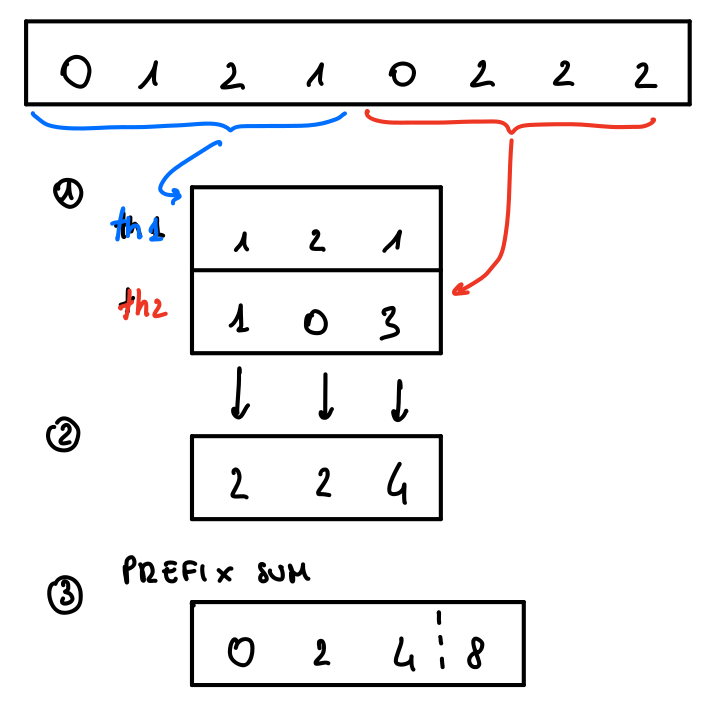
\includegraphics[scale=0.15]{index_to_pointers.png}
	\caption{Index to pointers}
	\label{index_to_pointers}
\end{figure}

\subsection{Pointers to index}
\label{pnt-to-idx}
Operazione inversa di \emph{index to pointers}. Il vettore risultante è ordinato. Può essere implementato assegnando ad ogni blocco di thread un elemento del vettore delle frequenze da espandere. 

L'algoritmo è illustrato in Figura~\ref{pointers_to_index}. 

\begin{figure}[t]
    \centering
	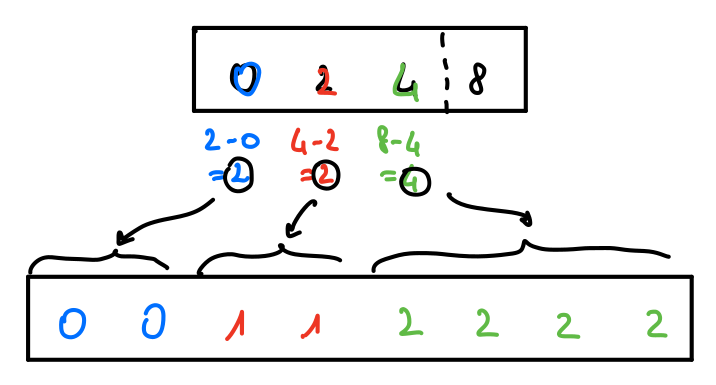
\includegraphics[scale=0.15]{pointers_to_index.png}
	\caption{Pointers to index}
	\label{pointers_to_index}
\end{figure}

Sperimentalmente si nota che il numero ottimale di thread per blocco è $1$.
